\documentclass[a4paper,12pt]{article}
\usepackage{amsfonts}
\usepackage{amssymb}
\usepackage{amsmath}
\usepackage{eurosym}
\usepackage{latexsym}
\usepackage{graphicx}
\usepackage{longtable}
\usepackage{portland}
\usepackage{lscape}
\usepackage[onehalfspacing]{setspace}
\usepackage{footmisc}
\usepackage{fancyhdr}
\usepackage{hyphenat}
\usepackage{rotating}
\usepackage[USenglish]{babel}
\usepackage{array}
\usepackage{tabularx}
\usepackage{chicago}
\usepackage{theorem}
\usepackage{multirow}
\usepackage{epstopdf}
\usepackage[left=1in,right=1in,top=1in,bottom=1in]{geometry}

\setcounter{MaxMatrixCols}{10}

\newtheorem{theorem}{Theorem}
\newtheorem{acknowledgement}[theorem]{Acknowledgement}
\newtheorem{algorithm}[theorem]{Algorithm}
\newtheorem{assum}{Assumption}
\newtheorem{axiom}[theorem]{Axiom}
\newtheorem{case}[theorem]{Case}
\newtheorem{claim}[theorem]{Claim}
\newtheorem{conclusion}[theorem]{Conclusion}
\newtheorem{condition}[theorem]{Condition}
\newtheorem{conjecture}[theorem]{Conjecture}
\newtheorem{corollary}[theorem]{Corollary}
\newtheorem{criterion}[theorem]{Criterion}
\newtheorem{definition}{Definition}
\newtheorem{example}[theorem]{Example}
\newtheorem{exercise}[theorem]{Exercise}
\newtheorem{lemma}[theorem]{Lemma}
\newtheorem{notation}[theorem]{Notation}
\newtheorem{problem}[theorem]{Problem}
\newtheorem{proposition}{Proposition}
\newtheorem{remark}[theorem]{Remark}
\newtheorem{solution}[theorem]{Solution}
\newtheorem{summary}[theorem]{Summary}
\newtheorem{observation}{Observation}
\newtheorem{result}{Result}

\pdfminorversion=6

\newcolumntype{L}[1]{>{\raggedright\arraybackslash}p{#1}} % linksbündig mit Breitenangabe
\newcolumntype{C}[1]{>{\centering\arraybackslash}p{#1}} % zentriert mit Breitenangabe
\newcolumntype{R}[1]{>{\raggedleft\arraybackslash}p{#1}} % rechtsbündig mit Breitenangabe

\begin{document}

\title{Assignment 2 \\ Solving RBC with VFI and EGM}
\author{Matthias Sch\"{o}n\thanks{CMR, University of Cologne; Albertus-Magnus-Platz; 50923 K\"{o}ln; Germany; E-mail:m.schoen@wiso.uni-koeln.de}}
\date{\today }
\maketitle

\begin{abstract}
This paper includes results and additional explanations to the second assignment of the course ECON 714-001 Quantitative Macro Theory by Jesus Fernandez Villaverde. In first section it contains a brief recall of main equations of the Real Business Cycle (RBC) model with endogenous labour supply. In the second part it shows the main results of performance of different implementation of Value Function Iteration (VFI) and Endogenous Grid Method (EGM) in terms of computational speed and accuracy of results. The last section provides a short description of the attached Fortran90 programming code.
\end{abstract}

\newpage \pagenumbering{arabic} \renewcommand{\thefootnote}{
\arabic{footnote}} \setcounter{footnote}{0}

\section*{Description of the RBC Model}

Consider following RBC model 
\begin{equation*}
\mathbb{V}\left( k,z\right) =\max [u\left( c,1-l\right) +\beta \mathbb{E}\mathbb{V}\left( k^{\prime},z^{\prime}\right)
\end{equation*}
where $c$ is consumption and $l$ is time spend in production.
The budget constraint is
\begin{equation*}
k^{\prime }=\left( 1-\delta \right) k+zf\left( k,l\right) -c.
\end{equation*}
The solution of the household problem using the separable CRRA preferences for consumption and leisure and a Cobb-Douglas production function lead to following set of equations.
\begin{equation}
\frac{1}{c}=\beta \mathbb{E}\mathbb{V}_{k}\left( k^{\prime },z^{\prime }\right) 
\label{VIII}
\end{equation}
\begin{equation*}
\psi l=\frac{1}{c}z\left( 1-\alpha \right) k^{\alpha}l^{-\alpha }
\end{equation*}
\begin{equation}
\mathbb{V}_{k}\left( k,z\right) =\frac{1}{c}\left[ \left( 1-\delta \right)+z\alpha k^{\alpha -1}l^{-\alpha }\right] 
\label{Envelope}
\end{equation}
Equation (\ref{VIII}) in combination with (\ref{Envelope}) yield the standard Euler Equation 
\begin{equation}
\frac{1}{c}=\beta \mathbb{E}\frac{1}{c^{\prime }}\left( \left( 1-\delta \right)+z^{\prime }\alpha \left( k^{\prime }\right) ^{\alpha -1}\left( l^{\prime}\right) ^{1-\alpha }\right).
\label{IX}
\end{equation}
Later this Euler equation is central to evaluate accuracy of computed solutions. From the previous problem set we already know that deterministic steady state values are 
\begin{eqnarray*}
k_{ss} &=&1.1909 \\
c_{ss} &=&0.4024 \\
y_{ss} &=&0.5096 \\
l_{ss} &=&1/3\\
V_{ss} &=&-26.6.
\end{eqnarray*}

\section*{Solution of RBC Model}

I compute all of the following results with the structural parameters of $\delta =0.09$, $\alpha =1/3$, $\psi =7.581$, $\beta =0.95$. Figure \ref{Policy_curr} show the Value Function and the Policy Functions for capital, labour and consumption. Those functions are derived from the benchmark VFI computed on 25,000 points on the capital grid and presented for each productivity state of the Markov process. In contrast to consumption and labour the policy function for capital show almost no curvature.  

\section*{Performance of VFI and EGM}

\subsection*{Grid size and Accuracy}

Main focus of this paper is not discussing the results of RBC model. It lies on the relative performance of different methods that solve this model. The first exercise is to compare performance by differing the amount of points the Value Function is evaluated on - in our case the the number of points in the capital grid. Figure \ref{Gridsize} shows the labour Policy Function for 178, 1780, and 17800 grid-points. In all different grids the distance between lowest and highest gridpoint is kept constant so that only the distance between the gridpoints is affected. The extreme coarse grid of 178 grid-points has easily observable kinks. These kinks are the result of big interpolation errors which occurs as the distance between grid-points the value function is known on is large. It is also easy to see that the kinks diminish as the number of grid-points increases. In the 17,800 grid they are graphically not unobservable even though they still exist.

Besides this graphically accuracy analysis of the computed policy I compute Euler Equation Errors (EEE) that become standard in the literature, cf. \citeN{aruoba06}. These EEE are derived from reshaping the Euler equation (\ref{IX}) in the following way
\begin{equation*}
EEE=1-c\beta \mathbb{E}\frac{1}{c^{\prime }}\left( \left( 1-\delta \right)+z^{\prime }\alpha \left( k^{\prime }\right) ^{\alpha -1}\left( l^{\prime}\right) ^{1-\alpha }\right) 
\label{EEE}
\end{equation*}
This error is a dimension free quantity expressing the optimization error as a fraction of current consumption. An error of $e_{1}=10^{-3}$, for instance, means the household would make a \$1 mistake for each \$1000 spent. These errors are expressed in units of base 10-logarithm which means that $-4$ is an error of $0.0001$. To see how big the mistakes of the solutions are i compute EEE forall gridpoints. Figure \ref{Error} shows a visualization of those errors for the benchmark VFI. As the EEE differ for each grid-point it is also convenient to report average and maximum EEE. Table \ref{AverageError} and \ref{MaximumError} show the results for all evaluated approaches of this paper.

One can see what we have already observed in figure \ref{Gridsize} and what is a standard feature of EEE. The higher the number of used grid-points the lower are the reported EEE. These errors are not fixed values but rely on the tolerance levels set in the code. So by increasing for example the convergence criterion from $10^{-6}$ to $10^{-4}$ the average EEE in the benchmark case increase from -4.6 to -3.2. This however would also lead to a decrease in the number of required iterations and therefore decrease the time until the VFI stops. There is a trade-off between computational accuracy and computational speed. As all evaluated approaches used the same convergence criterion they show similar results in terms of EEE what is necessary to have a fair evaluation based on computational time.
This performance of the different approaches in terms of computational speed is the core of this assignment. Table \ref{Time} shows the computing time until convergence of all evaluated approaches in this paper. In Column 2 we see that for the different amount of grid-points used in the benchmark VFI the speed until convergence is increasing linearly. So multiplying the amount of grid-points by 10 will also increase the computing time by a factor of 10. This is due to the fact that all calculation done by the computer is multiplied by 10. 

\subsection*{Varying Initial Guess}

In the benchmark VFI I set the initial guess of the value function to zero for all grid-points. A potentially better guess is to take the steady state value (-26.6) computed from steady state consumption and steady state labour.
\begin{equation*}
\mathbb{V}_{ss}=\frac{log(c_{ss})-\psi \frac{l_{ss}^{2}}{2}}{(1-\beta)} 
\end{equation*}
Comparing this value to the final Value Function in figure \ref{Policy_curr} we can see that matches the level quite well. Improving at least the level of the guess of the Value Function reduces the time until convergences by about 20\%, cf. table \ref{Time}. Even though this new initial guess is more precise in the level it is still a constant and has no slope. A potential additional improvement could be to give the guess a more similar slope. This requires, however, more computational effort. So compute first the value function obtained from the deterministic version of the problem (that is: solve for the value function without shocks) and then use it as initial guess for the problem with shocks. From the results in table \ref{Time} one see that this do not improve the speed. For all the following approaches I use the constant steady state level of the Value Function as initial guess.

\subsection*{Accelerator}

The next exercise is to use Policy Function Iteration. This accelerator also known as the Howards improvement algorithm skips the max operator in the Bellman several times and only updates the Value function for the given Policy Function and then iterate again on the value function once. In my example I skip the max operator 9 out of each 10 times. table \ref{Time} shows that this Policy Function Iteration enhances the speed of the code by a huge amount of time. In the 25,000 grid-point case it reduces the time compared to the benchmark VFI by almost 85\%. 

\subsection*{Stochastic Grid}

In this exercise I implement a stochastic grid scheme, cf. \citeN{Rust} for a Value function iteration, with 17820 grid-points around the deterministic steady state of capital. As one can see from table  \ref{Time} this approach does not speed up the value function and has almost the same property as the benchmark VFI. To be fair this is not a fair comparison as the advantage of the stochastic grid scheme are in higher dimensional problems and our standard RBC model has only two separate states. So the full power of the approach cannot be used.

\subsection*{Multi Grid}

Implementing a multi grid scheme, cf. \citeN{Chow}, for a Value function iteration, with the grid centered around deterministic steady state of capital and equally spaced is the most powerful approach in this setting. The different grid size are 100 capital grid points in the fi…rst grid, 1000 capital grid points in the second, and 25,000 capital grid points in the third. This stepwise implementing of the code reduces time until convergence to about 6.7\% of the time the benchmark VFI requires. 
I also combine the two previous approaches, multi grid and Howard, and get results even faster. The code finishes in 2.7 seconds compared to 110 seconds for benchmark VFI. I also run once the RBC model for 250,000 grid-points and it finishes in only 7.2 seconds. I used in this case 4 grids with (100, 1000, 25,000, 250,000). 

\subsection*{Endogenous Grid method}

In the last exercise I implement the code outline by \citeN{Barillas07}. Results are promising as this approach are also reduces the time compared to the benchmark VFI by a lot. For 1780 grid-points the time is reduced to only 15.8\%. For higher number of grid-points I face some problems with my numerical solver (zbrent - taken from Numerical Recipes) of the nonlinear equation that is required in this code and the computation time is extended. As in the stochastic grid case one have to consider that this is also not the best example for the EGM as due to endogenous labour supply a numerical solver is still required. The true power EGM develops when no numerical solver is needed. 

\section*{Explaining the Fortran90 Code}

This last section shortly describes the structure of the Fortran90 code in which I try to emphasizes modularity and functions\/subroutines. I implemented all of the above methods in one project called Assignment2. In this folder the main program is RBC\_Labour\_Main. To keep track of all the difference approaches I create this main file that only calls all other subroutines in which the actual iteration is provided and also to only compute once stuff that are needed for all approaches such like the subroutine sub\_RBC\_SteadyState that compute Steady State Values or subroutine sub\_RBC\_Error that computes average and maximum EEE. Most important in this main file are the settings that lead the whole code to the right method. There are five main options\{NGRIDS, INITIAL\_GUESS, HOWARD, STOCHASTIC, ENDOGENOUS\}. To choose one or a a combination\footnote{
Due to time constraint, the code do not allow the combination of ENDOGENOUS with the NGRIDS even if this would be a very promising option.}
change the according variable in the following way \vspace*{0.5cm} \\ 
\textit{! MULTIGRID SCHEME \newline
! NGRIDS:= How many grids to implement; nMultiGrid:= Define grid size in each step\newline
NGRIDS = 4\newline
allocate (nMultiGrid(NGRIDS))\newline
nMultiGrid = (\/100, 1000, 25000, 250000 \/)}\vspace*{0.5cm}
\textit{! INITIAL GUESS for Value Function\newline
! 1:= Constant Function equal Zeros\newline
! 2:= Constant Function equal to Steady State Value\newline
! 3:= Value function Obtained from the Deterministic Version of Problem\newline
INITIAL\_GUESS = 2}\vspace*{0.5cm}
\textit{! ACCELERATOR \- Policy Function Iteration\newline
! To use accelerator HOWARD:=1\newline
HOWARD = 1}\vspace*{0.5cm}
\textit{! STOCHASTIC GRID\newline
! STOCHASTIC:= 0 - Equally Spaced Grid\newline
! STOCHASTIC:= 1 - Randomly Distributed Grid-points \newline
STOCHASTIC = 0}\vspace*{0.5cm}
\textit{! ENDOGENOUS GRID\newline
! ENDOGENOUS:= 0 - VFI\newline
! ENDOGENOUS:= 1 - Endogenous Grid Method\newline
ENDOGENOUS = 0}\vspace*{0.5cm}

All parameter that are used in the code are included in the file RBC\_Parameter. Also important is the file sub\_RBC\_functions where I include all minor routines such as interpolation, grid generation ... .
\newpage

\bibliographystyle{chicago}
\bibliography{comparison}

\newpage

\begin{figure}[htb] \centering
\caption{RBC Value and Policy Functions}
\begin{tabular}{C{7.5cm} C{7.5cm}}
Value Function & Policy Function Capital\\
\includegraphics[width=7.5cm]{abbildungen/value_curr} & \includegraphics[width=7.5cm]{abbildungen/capital_curr} \\
Policy Function Consumption & Policy Function Labour\\
\includegraphics[width=7.5cm]{abbildungen/consumption_curr} & \includegraphics[width=7.5cm]{abbildungen/labour_curr} \\
\multicolumn{2}{p{14cm}}{{\footnotesize Solution to standard RBC model computed by VFI on a 25,000 capital grid around the deterministic steady state.}}
\end{tabular}
\label{Policy_curr}
\end{figure}
\begin{figure}[htb] \centering
\caption{Comparison Grid Size}
\begin{tabular}{C{4.5cm} C{4.5cm} C{4.5cm}}
178 Grid-points & 1780 Grid-points & 17800 Grid-points\\
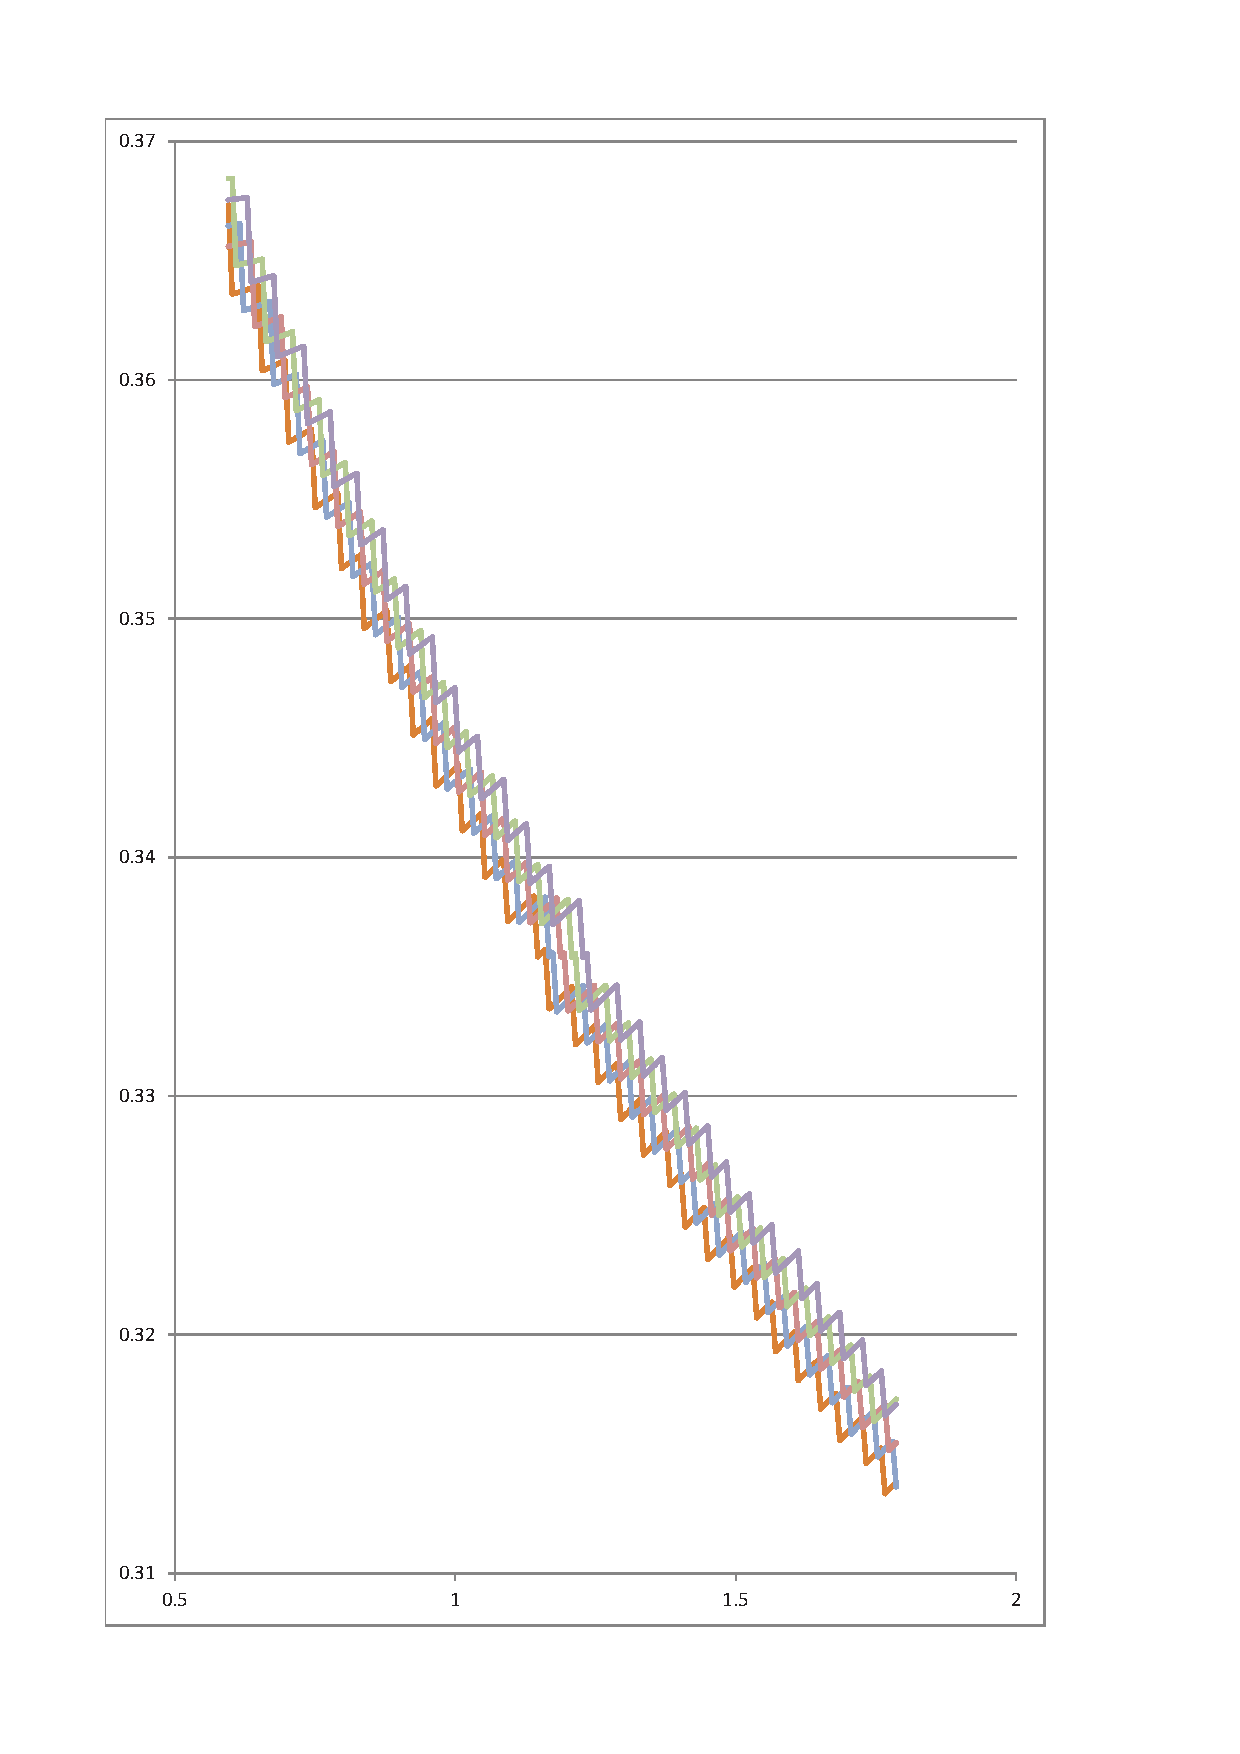
\includegraphics[width=4.5cm]{abbildungen/labour178} & 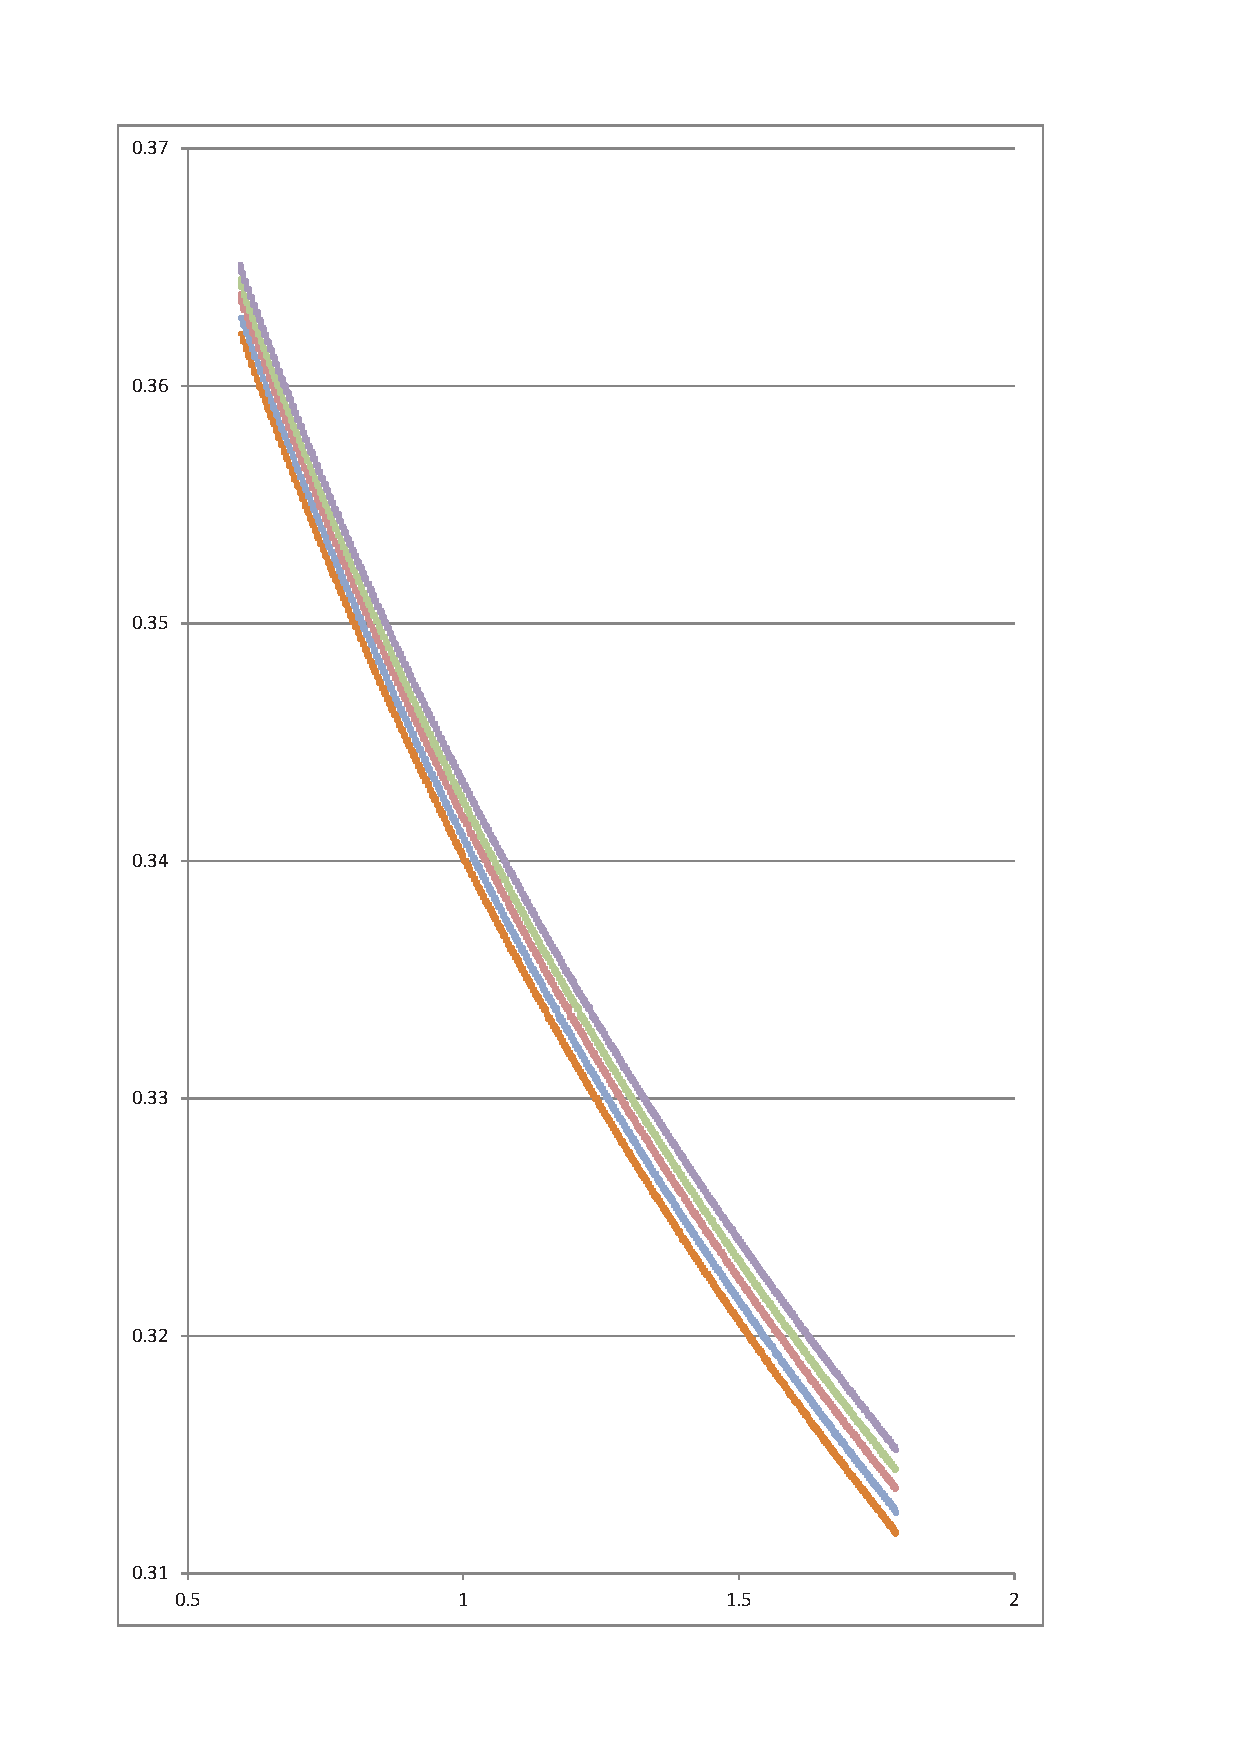
\includegraphics[width=4.5cm]{abbildungen/labour1780} & 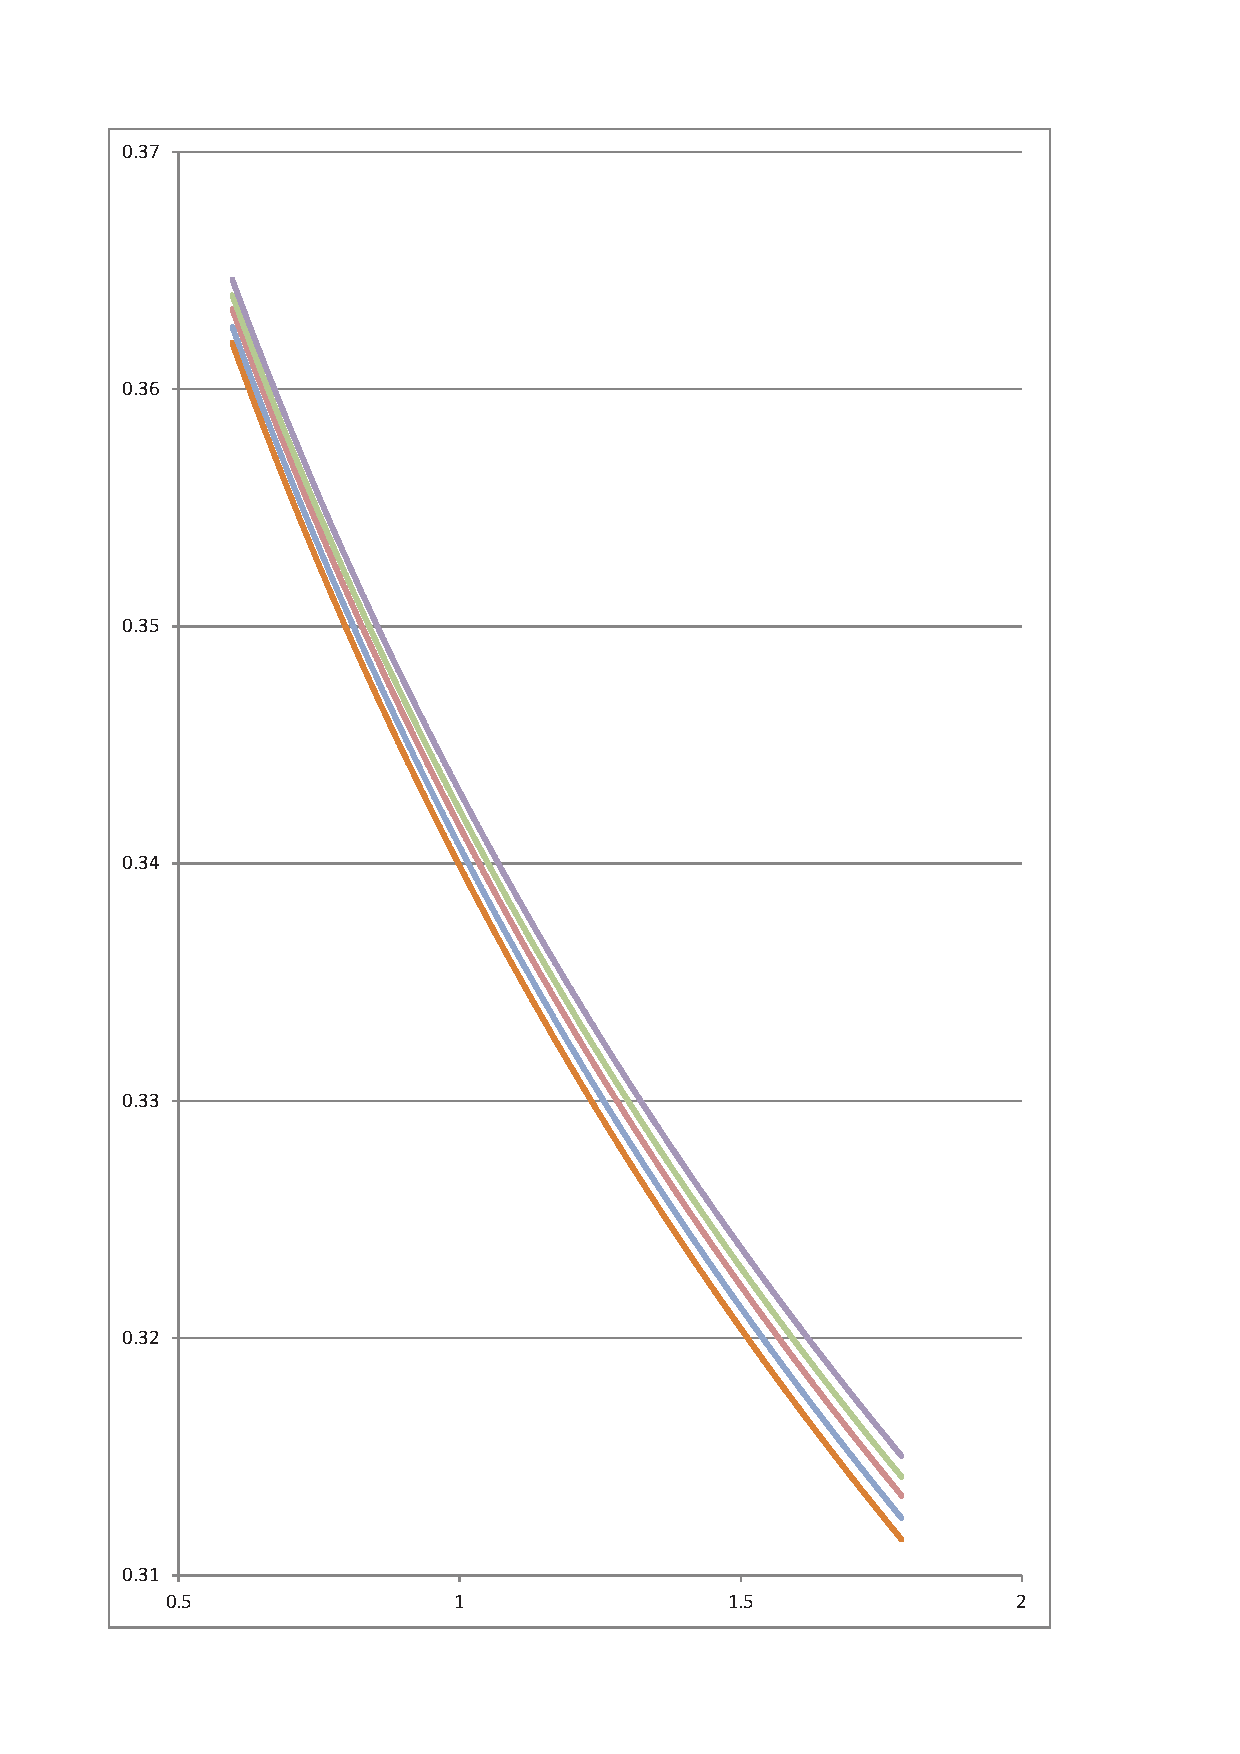
\includegraphics[width=4.5cm]{abbildungen/labour17800} \\
\multicolumn{3}{p{12cm}}{{\footnotesize Policy Function of Labour for 178, 1780 and 17,800 grid-points.}}
\end{tabular}
\label{Gridsize}
\end{figure}
\begin{figure}[htb] \centering
\caption{Euler Equation Error}
\begin{tabular}{c}
\includegraphics[scale=0.5]{abbildungen/error}\\
\multicolumn{1}{p{12cm}}{{\footnotesize EEE computed for all 25,000 gridpoint of capital grid holding the productivity state constant (z=1.0). Euler equation errors in units of base-10 logarithms.}}
\end{tabular}
\label{Error}
\end{figure}
\begin{table}[htb] \centering
\caption{Average Euler Equation Error}
\begin{tabular}{R{3.5cm}| C{2.5cm} C{2.5cm} C{2.5cm} C{2.5cm} }
&&&&\\
Number of Grid-points & 	Simple VFI &	Guess Level	& Guess	Slope	& Howard	\\ \hline	
178	  &-2.5 &-2.5	&-2.5	& -2.5	\\
1780	&-3.5	&-3.5	&-3.5	& -3.5	\\
17800	&-4.5	&-4.5	&-4.5	& -4.3	\\
25000	&-4.6	&-4.6	&-4.6	& -4.4	\\
\multicolumn{5}{c}{}\\
& Stochastic Grid &	Multi Grid (3)	& Multi Grid and Howard	& Endogenous Grid		\\ \hline				
178   &-2.23&	--  &	  --&	-2\\ 
1780  &-3.3 &	--	&   --& -3\\
17800 &-4.3 &	-4.5&	-4.2&	-4\\
25000 &-4.4 &	-4.6&	-4.3&	--\\ \hline	
\multicolumn{5}{p{12cm}}{{\footnotesize Average Euler equation errors are reported in units of base-10 logarithms.Code ends iteration when Value function deviation is lower than $10^{-6.}$}}
\end{tabular}
\label{AverageError}
\end{table}
\begin{table}[htb] \centering
\caption{Maximum Euler Equation Error}
\begin{tabular}{R{2.5cm}| C{2.5cm} C{2.5cm} C{2.5cm} C{2.5cm} }								
&&&&\\
Number of Grid-points & 	Simple VFI &	Guess Level	& Guess	Slope & Howard	\\ \hline	
178	  &-1.9	&-1.9	&-1.9	&-1.9\\
1780	&-2.8	&-2.8	&-2.8	&-2.8\\
17800	&-3.8	&-3.7	&-3.8	&-3.4\\
25000	&-3.9	&-3.9	&-3.9	&-3.5\\
\multicolumn{5}{c}{}\\
& Stochastic Grid &	Multi Grid (3)	& Multi Grid and Howard	& Endogenous Grid		\\ \hline	
178   &-1.28& --	& --	 &-1.2 \\
1780  &-2.3	& --	& --	 &-2   \\
17800 &-3	  &-3.7	& -3.1 &-2.5 \\
25000 &-3.1	&-3.9	& -3.3 &--   \\ \hline	
\multicolumn{5}{p{12cm}}{{\footnotesize Maximum Euler equation errors are reported in units of base-10 logarithms. Code ends iteration when Value function deviation is lower than $10^{-6.}$}}
\end{tabular}
\label{MaximumError}
\end{table}
\begin{table}[htb] \centering
\caption{Time until convergence}
\begin{tabular}{R{2.5cm}| C{2.5cm} C{2.5cm} C{2.5cm} C{2.5cm} }								
&&&&\\
Number of Grid-points & 	Simple VFI &	Guess Level	& Guess	Slope	& Howard	\\ \hline	
178	  & 0.96 & 0.76	&  1.18	&   0.09\\
1780	& 9.8	 & 7.8	&  11	  &   1.08\\
17800 &	98	 & 77	  & 110	  &  11.4\\
25000	&139	 &110	  & 156   &  15.8\\
\multicolumn{5}{c}{}\\
& Stochastic Grid &	Multi Grid (3)	& Multi Grid and Howard	& Endogenous Grid		\\ \hline
178   &  0.79	&  --	& --	& 0.26\\
1780  &  7.9	&  --	& --	& 1.2\\
17800	& 78    &	5.6 & 1.8 &	56\\
25000 & 110.3	& 7.4	& 2.5	& --\\\hline
\multicolumn{5}{p{12cm}}{{\footnotesize Time until convergence in seconds.}}
\end{tabular}
\label{Time}
\end{table}

\end{document}